\documentclass{article}
\usepackage{hyperref}
\usepackage{listings}
\usepackage{color}
\usepackage{xcolor}
\usepackage{geometry}
\usepackage{graphicx}
\usepackage{amsmath}
\usepackage{caption}
\usepackage{subcaption}
\usepackage[capitalise]{cleveref}
\usepackage{wrapfig}
\usepackage{amssymb}

\geometry{margin=1in}
\pdfminorversion=6

\newcommand\TODO[1]{\textcolor{red}{TODO: #1}}

\newcommand\header[2]{
    \begin{center}
        {\large
        UCSD CSE 167 Assignment #1: \\
        \vspace{0.3cm}
        \Large
        #2}
    \end{center}
}

\definecolor{dkgreen}{rgb}{0,0.6,0}
\definecolor{gray}{rgb}{0.5,0.5,0.5}
\definecolor{mauve}{rgb}{0.58,0,0.82}
\lstset{frame=tb,
        aboveskip=3mm,
        belowskip=3mm,
        showstringspaces=false,
        columns=flexible,
        basicstyle={\small\ttfamily},
        numbers=none,
        numberstyle=\tiny\color{gray},
        keywordstyle=\color{blue},
        commentstyle=\color{dkgreen},
        stringstyle=\color{mauve},
        breaklines=true,
        breakatwhitespace=true,
        tabsize=2
}

\lstdefinelanguage{Slang}{
  sensitive=true,
  morekeywords=[1]{
    if,else,for,while,do,switch,case,default,
    break,continue,return,discard,
    struct,class,interface,enum,
    static,const,uniform,
    in,out,inout,
    import,module,
    let,var
  },
  morekeywords=[2]{
    void,bool,
    int,int2,int3,int4,
    uint,uint2,uint3,uint4,
    float,float2,float3,float4,
    half,half2,half3,half4,
    float2x2,float3x3,float4x4,
    StructuredBuffer,RWStructuredBuffer,
    ByteAddressBuffer,RWByteAddressBuffer,
    Texture1D,Texture2D,Texture3D,TextureCube,
    RWTexture1D,RWTexture2D,RWTexture3D,
    SamplerState
  },
  morekeywords=[3]{
    shader,numthreads,
    SV_DispatchThreadID,SV_GroupID,SV_GroupThreadID,
    SV_Position,SV_Target,
    dot,cross,length,normalize,
    mul,lerp,clamp,saturate,
    min,max,abs,sqrt,pow,
    sin,cos,tan,asin,acos,atan,
    floor,ceil,round,frac,
    reflect,refract
  },
  morecomment=[l]{//},
  morecomment=[s]{/*}{*/},
  morestring=[b]"
}

\lstdefinestyle{slang}{
  language=Slang,
  basicstyle=\ttfamily\small,
  keywordstyle=[1]\color{blue},
  keywordstyle=[2]\color{teal},
  keywordstyle=[3]\color{violet},
  commentstyle=\color{gray},
  stringstyle=\color{orange},
  showstringspaces=false,
  columns=fullflexible,
  keepspaces=true,
  breaklines=true
}

% Taken from https://tex.stackexchange.com/questions/83085/how-to-improve-listings-display-of-json-files

\colorlet{punct}{red!60!black}
\definecolor{delim}{RGB}{20,105,176}
\colorlet{numb}{magenta!60!black}

\lstdefinelanguage{json}{
    basicstyle=\normalfont\ttfamily,
    numberstyle=\scriptsize,
    stepnumber=1,
    numbersep=8pt,
    showstringspaces=false,
    breaklines=true,
    frame=lines,
    tabsize=2,
    literate=
     *{0}{{{\color{numb}0}}}{1}
      {1}{{{\color{numb}1}}}{1}
      {2}{{{\color{numb}2}}}{1}
      {3}{{{\color{numb}3}}}{1}
      {4}{{{\color{numb}4}}}{1}
      {5}{{{\color{numb}5}}}{1}
      {6}{{{\color{numb}6}}}{1}
      {7}{{{\color{numb}7}}}{1}
      {8}{{{\color{numb}8}}}{1}
      {9}{{{\color{numb}9}}}{1}
      {:}{{{\color{punct}{:}}}}{1}
      {,}{{{\color{punct}{,}}}}{1}
      {\{}{{{\color{delim}{\{}}}}{1}
      {\}}{{{\color{delim}{\}}}}}{1}
      {[}{{{\color{delim}{[}}}}{1}
      {]}{{{\color{delim}{]}}}}{1},
}

\hypersetup{colorlinks=true}


\begin{document}

\header{4}{Physics-based Animation with Position-based Dynamics}

In this homework we will deal with animations. 
In particular we will deal with physics animation. 
We will do some rope and cloth animations along with collisions.
The method we will implement is based on ``position-based dynamics''.
A good reference for the method is the \href{https://matthias-research.github.io/pages/tenMinutePhysics/index.html}{Ten Minutes Physics}, from Matthias Müller who invented the position-based dynamics method. To save typing time, I will avoid introducing the method here: see my lectures and Müller's webpage for reference. 

If you know the drill: we will implement a constraint-based mass spring system with rods and cloth constraints, using a gather-based Jacobi iteration on GPU, with BVH collision detection and position-based friction.

\paragraph{Grading.} As usual, we will ask you to submit your code and results to us. For animation, it's much more difficult to match a reference frame-by-frame in general and we do not ask for that. A small floating point rounding error can propagate through the entire animation trajectory and lead to entire different animations (think of the famous ``butterfly effect'' -- many physical systems are ``chaotic'' and small perturbation can compound to large differences over time). We will look at your animation plus using some local unit tests (e.g., starting from some initial conditions and only test a few steps) to grade your code.

\section{Particle systems (5 pts)}

For the first part, we will implement a simple particle system. Each particle has a state of \lstinline{position} and \lstinline{velocity}.
We will use the \href{https://en.wikipedia.org/wiki/Semi-implicit_Euler_method}{symplectic Euler} method to update the position and velocity for each timestep. The particles are affected by a uniform gravity acceleration of $(0, -9.8, 0)$ everywhere. 
When a particle penetrate the floor (for this part, it is always at $y=-1$) after the update, we clip the y coordinate of the particle to be at the floor, and flip the $y$ component of velocity (and keep the other two unchanged) to simulate contact.
Just to make visualization easier, let's pretend the floor is at $y=-0.97$ in the simulation, so that the particles never land exactly on the floor.

Note that the algorithm is slightly different from the one we presented in the slide: we do not estimate the \emph{time of impact} and we do not reduce the time step when a collision is about to happen. We detect the collision ``after the fact''. This makes our collision not perfectly elastic and can introduce or lose energy. As a result you may see particles bouncing slightly higher or lower each time, which is completely normal.

\paragraph{Scene files.} Throughout this homework, we will use executable Python functions as our scene files (neat idea, no?). A scene file defines a \lstinline{make_scene} function that returns a dictionary. For this part, an example scene file is (\lstinline{hw4/particles.py}):
\begin{lstlisting}[language=python]
def make_scene():
    rng = np.random.default_rng(1)
    positions = (2.0 * rng.random((50, 3), dtype=np.float32) - 1.0) * 0.8
    positions[:, 1] += 0.2
    velocities = (2.0 * rng.random((50, 3), dtype=np.float32) - 1.0) * 0.05

    return {
        'positions': positions,
        'velocities': velocities,
        'show_particles': True,
        # The planes are stored as (a, b, c, d)
        # where ax+by+cz=d
        'planes': np.array([
            [0.0, 1.0, 0.0, -1.0],
        ], dtype=np.float32),
        # Camera configuration
        'cam_pos': (1.5, 0.1, -1.0),
        'cam_target': (0.0, -0.5, 0.0),
        'cam_up': (0.0, 1.0, 0.0)
    }
\end{lstlisting}
The comments of the constructor of the class \lstinline{HW4App} in \lstinline{hw4_app.py} has a more detailed description of what a scene should contain, but most of it may not make sense yet before we introduce the rest of the homework.

I have implemented the host part for you. It is in \lstinline{hw4/hw4.py}. Your task is to implement the aforementioned algorithm in \lstinline{hw4_1.slang}.

You can use the following command to test your code:
\begin{lstlisting}[language=bash]
uv run python main.py 4_1 scenes/hw4/particles.py
uv run python main.py 4_1 scenes/hw4/particles_2.py
uv run python main.py 4_1 scenes/hw4/particles_3.py
\end{lstlisting}
\textbf{Press space to start the animation.} Take some time to observe the chaos. ; )

I have put my rendering of the first scene in \lstinline{videos/hw_4_1_particles.mp4}.

Please send us your rendering produced by the following commands:
\begin{lstlisting}[language=bash]
uv run python main.py 4_1 scenes/hw4/particles_2.py -output outputs/hw_4_1_1.mp4 -duration 5 -fps 30
uv run python main.py 4_1 scenes/hw4/particles_3.py -output outputs/hw_4_1_2.mp4 -duration 5 -fps 30
\end{lstlisting}

\section{Elastic rope (18 pts)}

The previous part is mostly a warm up. Now we are going to do the real thing! We will implement a mass spring system using position-based dynamics. We assume there is only one connected mass spring (like \lstinline{o-o-o-o-o-o}, \lstinline{o} is mass and \lstinline{-} is spring). In the following I will assume you know the basics of mass spring systems and position-based dynamics. If you are confused, ask us!

\paragraph{Scene.} 
Here is a canonical scene file for 4.2. We generate an initial condition of a horizontal line. We also need to specify the edges for visualization. The edges are not used in the simulation: we assume there is only one connected mass spring. We then specify the ``inverse mass'' $\frac{1}{m}$. We use this over normal mass because in all of our simulation we only use the reciprocal. Finally we setup the rest lengths of the mass spring system.
\begin{lstlisting}[language=python]
def make_scene():
    count = 24
    # A horizontal line at y=0.6
    positions = np.zeros((count, 3), dtype=np.float32)
    positions[:, 0] = np.linspace(0.0, 1.8, count)
    positions[:, 1] = 0.6
    # For visualization purpose. Not used in simulation
    edges = np.stack([np.arange(count - 1),
                      np.arange(1, count)], axis=1).astype(np.uint32)

    inv_masses = np.ones(count, dtype=np.float32)
    inv_masses[0] = 0.0
    rest_lengths = np.linalg.norm(np.diff(positions, axis=0), axis=1).astype(np.float32)
    return {
        "positions": positions,
        "edges": edges,
        "inv_masses": inv_masses,
        "rest_lengths": rest_lengths,
        "substeps": 4, # number of timesteps we take per frame
        "iterations": 10, # number of Jacobi iterations we run per timestep
        # The planes are stored as (a, b, c, d)
        # where ax+by+cz=d
        'planes': np.array([
            [0.0, 1.0, 0.0, -1.0],
        ], dtype=np.float32),
        # Camera configuration
        'cam_pos': (1.5, -0.8, -1.5),
        'cam_target': (0.0, -0.4, 0.0),
        'cam_up': (0.0, 1.0, 0.0)
    }
\end{lstlisting}

\paragraph{Host code.} We have implemented the host code for you in \lstinline{hw4_2} in \lstinline{hw4/hw4.py}. Hopefully it is straightforward enough. The key logic is here, omitting some of the ugly argument passing:
\begin{lstlisting}
def step(command_encoder):
    nonlocal scratch_positions
    for _ in range(substeps):
        predict.kernel.dispatch(...)
        command_encoder.global_barrier()

        src, dst = app.positions, scratch_positions
        for _ in range(iterations):
            project.kernel.dispatch(...)
            command_encoder.global_barrier()
            src, dst = dst, src
        app.positions, scratch_positions = src, dst

        update.kernel.dispatch(...)
        command_encoder.global_barrier()
\end{lstlisting}

Your task is to implement the three kernels in Slang. All of them are launched to have one thread per vertex/particle. 

The \lstinline{predict} kernel applies gravity $(0, -9.8, 0)$ to the velocity and update the position (do NOT apply collision here yet like in 4.1). The \lstinline{old_positions} argument should store the positions before update, and the \lstinline{positions} and \lstinline{velocities} buffers store the updated position and velocity respectively.

The \lstinline{project} kernel does the actual Jacobi iteration: for each particle, we look at its neighbors (it either has one or two neighbors), compute the ``correction'' for each edge using the distance constraints, and update the position using the average of the correction vectors. 
For completeness, here's the correction vector for between particles $i$ and $j$ with positions $\mathbf{x}_i$ and $\mathbf{x}_j$, masses $m_i$ and $m_j$, and rest length $l_{ij}$:
\begin{equation}
\begin{aligned}
\Delta_{\mathbf{x}_i} &= \frac{w_i}{w_i + w_j} \left(\left\|\mathbf{d}\right\| - l_{ij}\right) \frac{\mathbf{d}}{\left\|\mathbf{d}\right\|} \\
\mathbf{d} &= \mathbf{x}_j - \mathbf{x}_i \\
w_k &= \frac{1}{m_k}.
\end{aligned}
\end{equation}
Also note that each Jacobi iteration uses \lstinline{positions_in} as input and write to \lstinline{positions_out}. 

The \lstinline{update} kernel clip the position against the floor at $y=-0.97$ and reconstruct the velocity using the clipped positions, to simulate a simplified contact scheme (we will later implement a more elaborated contact mechanism and remove this little hack). Note that the \lstinline{old_positions} buffer stores the position at the beginning of the timestep and should be the one you use to reconstruct the velocity.

Note that when a node has \lstinline{inv_masses[i] == 0} (i.e., infinite mass), it should not be moved at all.

Implement the three kernels in \lstinline{hw4/hw4_2.slang}. You can use the following commands to test your code:
\begin{lstlisting}[language=bash]
uv run python main.py 4_2 scenes/hw4/rope.py
uv run python main.py 4_2 scenes/hw4/catenary.py
uv run python main.py 4_2 scenes/hw4/crazy_rope.py
uv run python main.py 4_2 scenes/hw4/coil.py
\end{lstlisting}
I provided my own rendering of the first scene at \lstinline{videos/hw_4_2_rope.mp4}.

Please send us your rendering produced by the following commands:
\begin{lstlisting}[language=bash]
uv run python main.py 4_2 scenes/hw4/catenary.py -output outputs/hw_4_2_1.mp4 -duration 5 -fps 30
uv run python main.py 4_2 scenes/hw4/crazy_rope.py -output outputs/hw_4_2_2.mp4 -duration 5 -fps 30
uv run python main.py 4_2 scenes/hw4/coil.py -output outputs/hw_4_2_3.mp4 -duration 5 -fps 30
\end{lstlisting}

Play with some of the scene parameters yourself. It's useful to gain some intuitions of how these parameters affect the animation. Do this for each part later.

\section{Cloth (18 pts)}

Next let's use our previous code to handle clothes. The only difference between clothes and ropes are the topology. We will model a cloth as a 2D regular grid and store the particles in our regular 1D \lstinline{positions} array. Each vertex represents a 3D position. The discretization of the cloth is parameterized by \lstinline{grid_size} (two integers) and \lstinline{spacing} (two floats). \lstinline{grid_size} specifies how many vertices/particles we have in each dimension. \lstinline{spacing} specifies how far away they are from each other in each dimension. 

For each vertex at integer index $(x, y)$, cloth introduces three types of constraints: 
\begin{enumerate}
\item The \emph{structural} constraint preserves distances between $(x, y)$ and its immediate four neighbors $(x \pm 1, y)$ and $(x, y \pm 1)$. The rest length can be calculated from the \lstinline{spacing} parameter. 
\item The \emph{shearing} constraint preserves distances between $(x, y)$ and its four diagonal neighbors $(x \pm 1, y \pm 1)$ and $(x \pm 1, y \mp 1)$.
\item The \emph{bending} constraint preserves distances between $(x, y)$ and its four distance-2 neighbors $(x \pm 2, y)$ and $(x, y \pm 2)$.
\end{enumerate}

The host code for this part is almost identical to the previous part. We launch one thread per cloth vertex as before. The cloth vertices are arranged in row-major format, i.e., given a \lstinline{tid} you convert it into the $(x, y)$ integer index with \lstinline{(tid % grid_size.x, tid / grid_size.x)}.

Even better, the \lstinline{predict} and \lstinline{update} kernels are also identical to the previous part. So the only thing you need to implement is the \lstinline{project} kernel. I will let you figure out the rest! Implement the kernel in \lstinline{hw4/hw4_3.slang}.

You can use the following commands to test your code:
\begin{lstlisting}[language=bash]
uv run python main.py 4_3 scenes/hw4/cloth.py
uv run python main.py 4_3 scenes/hw4/hammock.py
uv run python main.py 4_3 scenes/hw4/spin_cloth.py
uv run python main.py 4_3 scenes/hw4/big_cloth.py
\end{lstlisting}
I provided my own rendering of the first scene at \lstinline{videos/hw_4_3_cloth.mp4}.

Please send us your rendering produced by the following commands:
\begin{lstlisting}[language=bash]
uv run python main.py 4_3 scenes/hw4/hammock.py -output outputs/hw_4_3_1.mp4 -duration 5 -fps 30
uv run python main.py 4_3 scenes/hw4/spin_cloth.py -output outputs/hw_4_3_2.mp4 -duration 5 -fps 30
uv run python main.py 4_3 scenes/hw4/big_cloth.py -output outputs/hw_4_3_3.mp4 -duration 5 -fps 30
\end{lstlisting}

\section{General mass-spring systems using sparse matrices (18 pts)}

\begin{figure}[t]
\centering
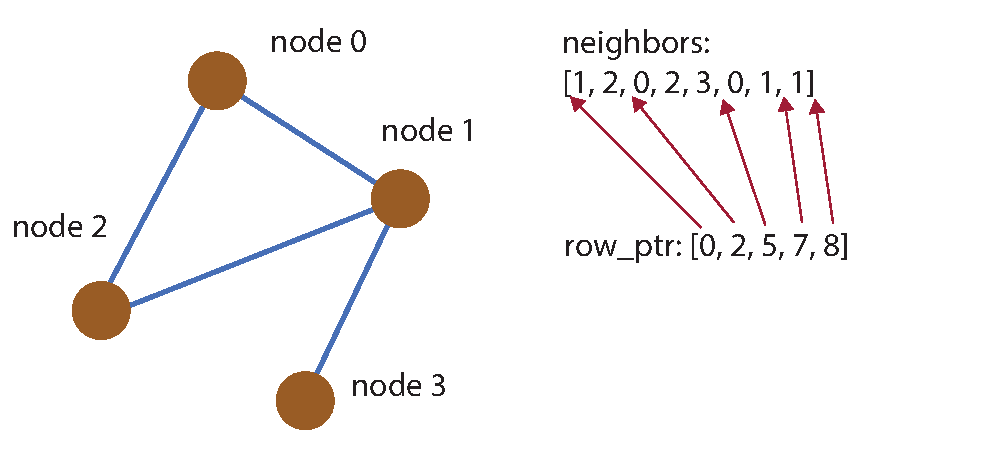
\includegraphics[width=0.5\linewidth]{imgs/csr_matrix.pdf}
\caption{To store the edges of a graph, we use two arrays: \lstinline{neighbors} and \lstinline{row_ptr}. \lstinline{neighbors} is a flattend 1D array that records the indices of the neighbor of each node. In this case, node 0 has neighbors of node 1 and node 2 (stored as \lstinline{1, 2} in the array), node 1 has neighbors of nodes 0, 2, and 3 (stored as \lstinline{0, 2, 3} in the array). For each node \lstinline{i}, to grab the neighbors, we use the \lstinline{row_ptr[i]} array to index into the neighbors array. \lstinline{row_ptr[i+1]} then marks the end (non-inclusive) of the neighbor list of node \lstinline{i}.}
\label{fig:csr_matrix}
\end{figure}

Next we will combine our cloth code and rope code to handle pretty much arbitrary mass-spring topology. The main difference is how we get the edges: previously we assume a particular topology like a chain of nodes or a 2D grid of nodes. Now we can have a general graph. We represent a graph's \href{https://en.wikipedia.org/wiki/Adjacency_matrix}{adjacency matrix} using a ``Compressed Sparse Row'' (CSR) format. It sounds fancy but it really just an array and an array of pointers. See \cref{fig:csr_matrix}. We further store the rest length of the edge in the \lstinline{neighbor_rest} array. 

Given the CSR matrix, we can easily extend our cloth simulation code to handle arbitrary topology. Even better, the Jacobi iteration loop on the host side remains almost unchanged (we just need to pass the CSR matrix). 

Our scenes provide the edges and we have provided the code to build the CSR matrix given the edges. In particular, the scene constructs a list of edges like this:
\begin{lstlisting}[language=python]
edges = []
for r in range(1, rings + 1):
    for s in range(spokes):
        edges.append((index(r - 1, s), index(r, s)))
        edges.append((index(r, s), index(r, s + 1)))
edges = np.array(edges, dtype=np.uint32)
\end{lstlisting}
We then turn this edge list into a CSR matrix using the \lstinline{build_csr} function in \lstinline{hw4/hw4.py}. The rest is similar to the previous parts.

Your task is, again, to implement the \lstinline{project} kernel in \lstinline{hw4/hw4_4.slang}. Use the following commands to test your code:
\begin{lstlisting}[language=bash]
uv run python main.py 4_4 scenes/hw4/spider_web.py
uv run python main.py 4_4 scenes/hw4/suspension_bridge.py
uv run python main.py 4_4 scenes/hw4/branching_pendulum.py
uv run python main.py 4_4 scenes/hw4/big_hammock.py
\end{lstlisting}

Please send us your rendering produced by the following commands:
\begin{lstlisting}[language=bash]
uv run python main.py 4_4 scenes/hw4/suspension_bridge.py -output outputs/hw_4_4_1.mp4 -duration 5 -fps 30
uv run python main.py 4_4 scenes/hw4/branching_pendulum.py -output outputs/hw_4_4_2.mp4 -duration 5 -fps 30
uv run python main.py 4_4 scenes/hw4/big_hammock.py -output outputs/hw_4_4_3.mp4 -duration 5 -fps 30
\end{lstlisting}

\section{Contact and friction with simple static colliders (18 pts)}
So far we only deal with the distance constraints between the masses in the mass spring system. Now let's add collision with simple primitives like spheres and (infinite) planes. We also assume that the spheres and planes are static, just to make things easier. The spheres and planes form \emph{signed distance functions} that we can use to detect whether a point is inside or outside of an object, and if it is inside, how far have we penetrated into the object. (For planes, we assume that it is ``one-sided'', meaning that one side of the plane is completely ``inside'' the object.)

The position-based dynamics method can be easily extended to handle contact and friction. In addition to \lstinline{predict}, \lstinline{project}, and \lstinline{update}, we add a \lstinline{detect_collision} kernel between \lstinline{predict} and \lstinline{project}. If after the position prediction, our current position evaluates to negative for any of our signed distance function colliders, a collision has happened. If we detect a potential collision (within contact margin), inside \lstinline{project}, we add more corrections inside the Jacobi iteration after the distance constraints projection to move the particles outside of the colliders and apply tangential movements as friction. Inside \lstinline{update}, we can also now remove the hacky clipping against $y=-0.97$. \lstinline{predict} remains unchanged. We now detail each part.

\paragraph{Collision detection.} The interface to the collision detection kernel looks like this:
\begin{lstlisting}[language=Slang]
[shader("compute")]
[numthreads(64, 1, 1)]
void detect_collision(uint tid : SV_DispatchThreadID,
                      StructuredBuffer<float3> positions,
                      StructuredBuffer<float> inv_masses,
                      // Plane stores (a, b, c, d) where ax+by+cz=d
                      // a, b, c are normalized to a unit 3D vector
                      StructuredBuffer<float4> planes,
                      // Sphere stores center (xyz) + radius (w)
                      StructuredBuffer<float4> spheres,
                      // Contact plane: dot(n, x) = d, with unit normal n
                      RWStructuredBuffer<float4> contact_planes,
                      uniform uint particle_count,
                      uniform uint plane_count,
                      uniform uint sphere_count,
                      // How much should we shift the generated 
                      // contact plane in the normal direction
                      // (similar to how we shifted the floor by 0.03
                      //  earlier)
                      uniform float collision_distance,
                      // When the signed distance function
                      // evaluates to a value below 
                      // contact_margin + collision_distance
                      // (even when it's positive), we count the
                      // particle to be inside the collider and
                      // a collision event has happened.
                      uniform float contact_margin)
\end{lstlisting}
Each particle corresponds to one thread. The main output of this kernel is the array \lstinline{contact_planes}, which has the same size as the number of particles. The \lstinline{contact_planes} store the tangent plane of the recorded contact event using the same format as the input planes. If there is no contact, I store $(0, 0, 0, 0)$ in my implementation, but you can do whatever you want. A particle can be inside of many colliders, and in this homework we only store the collider with the smallest signed distance value at the particle position\footnote{In real production simulators, the collision are typically stored as a list of pairs between the colliders and the collidees. Some systems such as NVIDIA Flex/PhysX store up to 6 contact planes per particle, but how they choose these colliders is not detailedly documented.}. Note that for spheres, storing a contact plane is a local approximation, 

So, inside this kernel, for each particle, you test through all the colliders (spheres and planes), evaluate their signed distance functions, record the smallest signed distance. If the smallest signed distance is smaller than \lstinline{contact_margin + collision_distance}, we record the collision event by storing the contact plane. The contact plane is shifted by \lstinline{collision_distance} in the normal direction (\lstinline{plane.w += collision_distance}).

\paragraph{Projecting contact.}
A contact event generates two types of constraints/corrections. We apply the contact correction \emph{after} the correction for the distance constraints between particles have been applied inside one Jacobi iteration. In below when we say the current position $\mathbf{x}$ it refers to the position inside one Jacobi iteration after the distance constraints correction.

One of the two constraints/correction is in the normal direction, and another one is in the tangential direction. We get the normal direction from the contact plane (\lstinline{n=plane.xyz}), and we can get the tangential direction by projecting the vector between the current position $\mathbf{x}$ in the Jacobi iteration and the old position on to the tangent plane (\lstinline{tangent = x - old_position - dot(x - old_position, n) * n}). We first apply the normal correction, then the tangential correction.

For the normal direction contact, the constraint is an \emph{inequality constraint}: our position should be above of the contact plane. Therefore the correction for the normal direction is to first compute a ``penetration depth'' using the current position $\mathbf{x}$ and the contact plane by measuring the signed distance between $\mathbf{x}$ and the contact plane, and retain only the negative values. For the correction of the normal direction contact constraint, we then move in the normal direction by the penetration depth to project the position outside of the contact plane.

For the tangential direction, friction will apply. There are two types of frictions. First is \emph{static friction}, which completely stops the motion in the tangential direction. Static friction can only resist a limited amount of motion. If the tangent displacement is too long, we switch to \emph{kinetic friction}, which only slows down the motion in the tangential direction. We use \lstinline{static_friction} and \lstinline{kinetic_friction} to decide how much tangential correction is applied. Both correction are proportional to the penetration depth.
In pseudocode it looks like:
\begin{lstlisting}[language=Python]
// penetration = penetration depth, a positive scalar
if (tangent_len <= static_friction * penetration) {
    // static friction, completely kills the tangential motion
    // by applying a correction to x in the negative tangent direction
    // move back to the old position in the tangent direction completely
} else {
    // kinetic friction, slows down the tangential motion
    // also by applying a correction to x in the negative tangent direction
    // move back to the old position in the tangent direction
    // by the amount of kinetic_friction * penetration
}
\end{lstlisting}
Technically friction is not a constraint, but it can also be incorporated easily into the Jacobi iteration and modifies the position.

Sorry if I didn't explain it completely clear. Contact and friction is fully of implementation-specific approximations and heuristics, and pretty much everyone does it slightly differently. Let us know if there is any detail unclear.

As usual, we have implemented the host part for you. Your task is to implement the \lstinline{detect_collision}, \lstinline{project}, and \lstinline{update} functions using the method as described above. 

Use the following commands to test your code:
\begin{lstlisting}[language=bash]
uv run python main.py 4_5 scenes/hw4/simple_colliders.py
uv run python main.py 4_5 scenes/hw4/rope_collide.py
uv run python main.py 4_5 scenes/hw4/cloth_tunnel.py
uv run python main.py 4_5 scenes/hw4/composite_collide.py
uv run python main.py 4_5 scenes/hw4/suspended_cloth_collide.py
\end{lstlisting}

I have provided my rendering of the first scene in \lstinline{videos/hw_4_5_simple_colliders.mp4}.

Send us your rendering produced by the following commands:
\begin{lstlisting}[language=bash]
uv run python main.py 4_5 scenes/hw4/rope_collide.py -output outputs/hw_4_5_1.mp4 -duration 5 -fps 30
uv run python main.py 4_5 scenes/hw4/cloth_tunnel.py -output outputs/hw_4_5_2.mp4 -duration 5 -fps 30
uv run python main.py 4_5 scenes/hw4/composite_collide.py -output outputs/hw_4_5_3.mp4 -duration 5 -fps 30
uv run python main.py 4_5 scenes/hw4/suspended_cloth_collide.py -output outputs/hw_4_5_4.mp4 -duration 5 -fps 30
\end{lstlisting}

\section{Collision with triangle meshes using Bounding Volume Hierarchies (18 pts)}
Yes you hear it right. BVHes are back! It's perhaps not surprising that the signed distance function evaluation we do for the collision detection can be sped up using BVH as well. For this part we will handle collision with static triangle meshes. We will first explain collision with triangle meshes, then get back to how to use a BVH to speed it up.

Extending our previous approach to handle triangle meshes requires computing the signed distance function of a triangle mesh. This turns out to be a little bit tricky! Computing the \emph{unsigned} distance is easy: given a point, for each triangle, we can calculate the closest distance on the triangle. We then loop over all triangles and pick the minimal distance among all triangles. Checking whether a point is inside or outside of the triangle mesh is, however, slightly messy. Firstly, if the mesh is not \emph{closed}, then the notion of inside vs. outside becomes vague (there actually is a way to do this -- check out the concept of \emph{generalized winding number}). Secondly, if the mesh is \emph{closed}, checking whether a point is inside the mesh or not requires computing the winding number (remember Homework 1?). This can be done by using the same raycasting approach we did in Homework 1, but then you need to do real-time ray tracing just to figure out whether a particle is inside or outside a mesh.

Instead, we opt for a simpler approach. We first find the closest triangle using the \emph{unsigned} distance. Next, if the triangle is a potential contact target (distance is smaller than \lstinline{contact_margin + collision_distance}), we pretend the triangle is an infinite plane like the previous part, and compute the signed distance to that infinite plane. The rest is the same as previous part.

There is one last detail: how do we get the orientation of the triangle? A triangle technically has two normals, and using the wrong one can make us apply the wrong collision constraint. We make use of the vertex normals! We assume that the vertex normals themselves are properly oriented. Then we choose the triangle face normal that is on the same side as the vertex normal interpolated at the closest point on the triangle. Pseudocode wise it looks like this:
\begin{lstlisting}[language=Slang]
// Face normal
float3 ng = normalize(cross(p1 - p0, p2 - p0));
// Phong normal
float3 ns = normalize(b0 * n0 + b1 * n1 + b2 * n2);
if (dot(ng, ns) < 0.0) {
    ng = -ng;
}
// Use ng as the normal of our contact plane.
\end{lstlisting}
I recommend implement a version first without the BVH and test it on a smaller mesh.

Now the BVH: it is used to speedup the process of finding the closest triangle. For each particle, instead of looping over all the triangles, we traverse a BVH. We will use the stackless traversal we did in the previous homework. We first initialize the minimal distance to be \lstinline{contact_margin + collision_distance}. During the traversal, we can compute the distance between the particle position to the bounding volume: if the distance is larger than the minimal distance we found so far, we can safely skip this BVH node (using the skip index). If we reach a leaf node, we compute the distance to all triangles inside that leaf node, and update our minimal distance. 

And we are done! Turns out we only need to modify the \lstinline{detect_collision} kernel from last part. Everything else can stay the same!
To simplify things we assume there is only one mesh and one BVH. We have provided the BVH building code on the host as usual, and the data structure is basically the same as Homework 3.

As the other parts I have implemented the host code. The codes for computing the distance between a point and an axis-aligned bounding box (\lstinline{point_aabb_distance}) and the closest point on a triangle to a query point (\lstinline{closest_point_triangle}) are also provided. Your job is to implement \lstinline{detect_collision} and handle spheres, planes, and meshes.

Test your code using the following commands:
\begin{lstlisting}[language=bash]
uv run python main.py 4_6 scenes/hw4/cloth_low_poly_rock.py
uv run python main.py 4_6 scenes/hw4/cloth_bunny.py
uv run python main.py 4_6 scenes/hw4/rope_bunny.py
uv run python main.py 4_6 scenes/hw4/suspended_cloth_bunny.py
uv run python main.py 4_6 scenes/hw4/cloth_bunny_balls.py
\end{lstlisting}
I have provided my rendering of the first scene in \lstinline{videos/hw_4_6_cloth_low_poly_rock.mp4}.

As usual, please send us your rendering produced by the following commands:
\begin{lstlisting}[language=bash]
uv run python main.py 4_6 scenes/hw4/cloth_bunny.py -output outputs/hw_4_6_1.mp4 -duration 5 -fps 30
uv run python main.py 4_6 scenes/hw4/rope_bunny.py -output outputs/hw_4_6_2.mp4 -duration 5 -fps 30
uv run python main.py 4_6 scenes/hw4/suspended_cloth_bunny.py -output outputs/hw_4_6_3.mp4 -duration 5 -fps 30
uv run python main.py 4_6 scenes/hw4/cloth_bunny_balls.py -output outputs/hw_4_6_4.mp4 -duration 5 -fps 30
\end{lstlisting}

\section{Make your own scene (5 pts)}
Last stretch! As usual make your own scene for the last part. Drop cloth on weird meshes. Make weird rope animations. Weird topology mass spring systems. Anything you like! Submit both your scene (\lstinline{.py}) and the rendering video.


\end{document}

